\subsection{Resource Results}

%The big table!
% Please add the following required packages to your document preamble:
% \usepackage{multirow}
% \usepackage[table,xcdraw]{xcolor}
% If you use beamer only pass "xcolor=table" option, i.e. \documentclass[xcolor=table]{beamer}
\begin{table*}[t]
\centering
\caption{Table of Resource Consumption}
\label{tab:the_big_table}
\begin{tabular}{lllllllllllllllllllllll}
\cline{1-14}
\textbf{Benchmarks}          &                    & \multicolumn{12}{l}{\textbf{Resource Usage}}                                                            & \multicolumn{9}{l}{Error Resilience}                                                  \\ \cline{1-1} \cline{3-14}
                             &                    & \multicolumn{4}{l}{\textit{Original}} & \multicolumn{4}{l}{\textit{StitchUp}} & \multicolumn{4}{l}{DMR} & \multicolumn{3}{l}{Original} & \multicolumn{3}{l}{StitchUp} & \multicolumn{3}{l}{DMR} \\ \cline{1-1} \cline{3-6}
                             &                    & LUT     & REG     & DSP    & Power    & LUT     & REG     & DSP    & Power    & LUT & REG & DSP & Power & Time    & Data    & Caught   & Time    & Data    & Caught   & Time  & Data  & Caught  \\ \cline{1-1} \cline{3-3}
{\color[HTML]{333333} adpcm} &                    &         &         &        &          &         &         &        &          &     &     &     &       &         &         &          &         &         &          &       &       &         \\ \cline{1-1} \cline{3-3}
                             &                    &         &         &        &          &         &         &        &          &     &     &     &       &         &         &          &         &         &          &       &       &         \\ \cline{1-1} \cline{3-3}
                             & \multirow{-6}{*}{} &         &         &        &          &         &         &        &          &     &     &     &       &         &         &          &         &         &          &       &       &         \\ \cline{1-3}
\end{tabular}
\end{table*}

\begin{table*}[t]
\centering
\caption{Table of Error properties}
\label{tab:errorTable}
\begin{tabular}{llllllllllllllllllll}
\cline{1-3}
\textbf{}                    &                    & \textbf{}     &          &            &            &            &             &       &       &         &       &       &      &       &       &      &       &       &      \\ \cline{1-1} \cline{3-5}
\textbf{}                    &                    & \multicolumn{3}{l}{\textit{Original}} & \multicolumn{3}{l}{\textit{StitchUp}} & \multicolumn{3}{l}{DMR} & \multicolumn{3}{l}{} & \multicolumn{3}{l}{} & \multicolumn{3}{l}{} \\ \cline{1-1} \cline{3-5}
                             &                    & Time          & Data     & Caught     & Time       & Data       & Caught      & Time  & Data  & Caught  &       &       &      &       &       &      &       &       &      \\ \cline{1-1} \cline{3-3}
{\color[HTML]{333333} adpcm} &                    &               &          &            &            &            &             &       &       &         &       &       &      &       &       &      &       &       &      \\ \cline{1-1} \cline{3-3}
                             &                    &               &          &            &            &            &             &       &       &         &       &       &      &       &       &      &       &       &      \\ \cline{1-1} \cline{3-3}
                             & \multirow{-6}{*}{} &               &          &            &            &            &             &       &       &         &       &       &      &       &       &      &       &       &      \\ \cline{1-3}
\end{tabular}
\end{table*}

\begin{figure}[h]
\centering
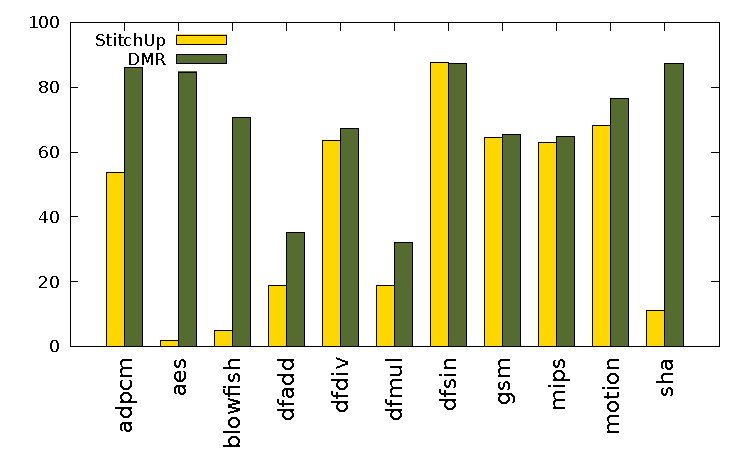
\includegraphics[width=2.5in]{./graphs/chstone_luts_24_09_2015.pdf}
\caption{Luts for the CHStone benchmark}
\label{fig:luts_result}
\end{figure}

\begin{figure}[h]
\centering
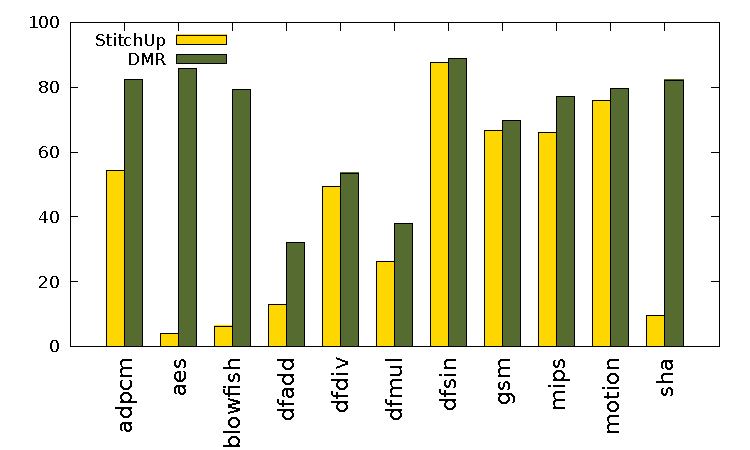
\includegraphics[width=2.5in]{./graphs/chstone_reg_24_09_2015.pdf}
\caption{REGs for the CHStone benchmark}
\label{fig:regs_result}
\end{figure}

\subsection{Power Results}

\begin{figure}[h]
\centering
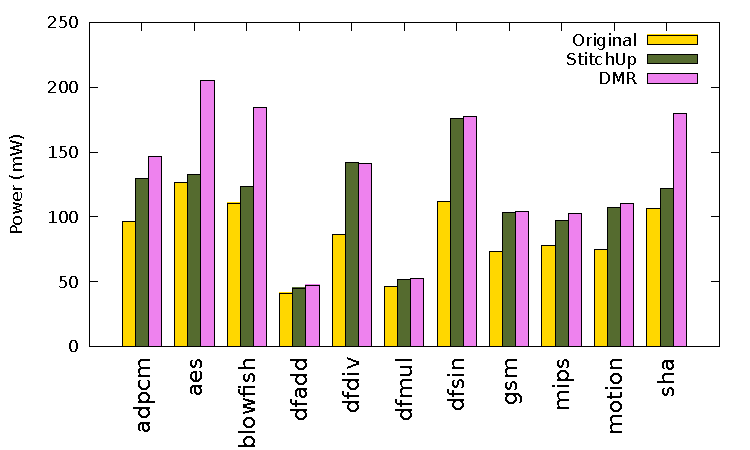
\includegraphics[width=2.5in]{./graphs/chstone_absolute_power_24_09_2015.pdf}
\caption{Power for the CHStone benchmark}
\label{fig:power_result}
\end{figure}

\subsection{Fault Injection Results}
